\documentclass[12pt,a4paper]{article}
%\usepackage{cwtex}
%\usepackage{fancyvrb}
\usepackage{graphicx}
%\usepackage{CJK} %使用CJK套件
\usepackage{CJKutf8} %使用CJK套件
\usepackage{comment}
\usepackage{hyperref} % 最好保证 hyperref 是最后加载的宏包
\hypersetup{%
%  dvipdfmx,% 设定要使用的 driver 为 dvipdfmx
  dvips,% 设定要使用的 driver 为 dvipdfmx
  unicode={true},% 使用 unicode 来编码 PDF 字符串
  pdfstartview={FitH},% 文档初始视图为匹配宽度
  bookmarksnumbered={true},% 书签附上章节编号
  bookmarksopen={true},% 展开书签
  pdfborder={0 0 0},% 链接无框
  pdftitle={IPAQ 使用心得},
  pdfauthor={descent},
  pdfsubject={IPAQ 3870},
  pdfkeywords={PDA},
  pdfcreator={ps2pdf},
  pdfproducer={PDF 制作程序},% 这个好像没起作用?
}

\parindent=0cm
\parskip=20pt

\begin{document}
\begin{CJK}{UTF8}{cwmu} %開始CJK環境,設定編碼,設定字體
\renewcommand{\contentsname}{目錄}
\renewcommand{\tablename}{表}
\renewcommand{\figurename}{圖}
\renewcommand{\listtablename}{表格目錄}
\renewcommand{\listfigurename}{圖目錄}
%\begin{htmlonly}
% 標題頁
\begin{titlepage}
\fontsize{30}{30pt plus.5pt minux.4pt}\selectfont
\noindent
%Document Title:\\[6pt]
使用 Autoconf, Automake, Libtool

\fontsize{14}{20pt plus.5pt minux.4pt}\selectfont
\par\vfill\noindent

Author: descent\\
%文件版本:$Revision$
%文件版本:$Id$

\today


\end{titlepage}

%\end{htmlonly}

%\begin{title}


%\end{title}

\newpage

\tableofcontents
\newpage

%\ctxfoff

\section{更換 bootloader}
首先到
http://familiar.handhelds.org/releases/v0.8.2/install/download.html
下載必須的檔案。
我下載的是 bootopie-h3600.tar,
untar 之後有以下檔案。

\begin{verbatim}
BootBlaster_1.19.exe       md5sums
bootldr-sa-2.21.12.bin     opie-image-h3600-20050407124742.rootfs.jffs2
bootldr-sa-2.21.12.bin.gz  reflash.ctl
\end{verbatim}

\verb+BootBlaster_1.19.exe+ 這是用來安裝新的 bootloader,
可以 boot wince, linux。

bootldr-sa-2.21.12.bin 便是 bootloader。

opie-image-h3600-20050407124742.rootfs.jffs2 這是 linux image file,
要透過 bootloader 載入。

\section{使用 minicom}
執行 minicom, minicom 需要 lrzsz 套件,
若是在執行 minicom 進行 xmodem, ymodem, zmodem 有問題時,
檢查 lrzsz 是否安裝。

IPAQ 接在 /dev/ttyS0 (com1),
接在 /dev/ttyS1 (com2) 好像不能 work。

以下為我的 Serial port setup   

\begin{tabular}{ccccl}
A & - &   Serial Device &     : & /dev/ttyS0\\
B & - & Lockfile Location  &   : & /var/lock\\
C & - &  Callin Program    & : &  \\
D & - &  Callout Program   & : &  \\
E & - &  Bps/Par/Bits    &   : & 115200 8N1\\
F & - & Hardware Flow Control & : & No\\
G & - & Software Flow Control &:& No   \\
\end{tabular}

如此一來, 就可以透過 minicom 和 iPAQ 連線,
當然,必須先安裝 familiar linux distribution。

\section{IPAQ 的 bootloader 指令}

在 familiar bootload 下, type
load root,
可以載入一個 jffs2 的 root file system。
也可以用來載入之前備份的 wince image。


bootstrap-v0.7.2-h3600.tar untar 此檔案會得到一個可以開機的 jffs2 image。
沒有 GUI 圖形環境。

\section{compile QT/E, OPIE, QTOPIA}
\subsection{OPIE}
patch qt/e
\begin{verbatim}
cd $QTDIR; cat $OPIEDIR/qt/qte23x-all.patch | patch -p1
\end{verbatim}

或是

\begin{verbatim}
patch -p1 < $OPIEDIR/qt/qte237-all.patch 
\end{verbatim}

若是 compie QTOPIA 不用 patch qte-2.3.7,
\begin{verbatim}
ln -s $OPIEDIR/qt/qconfig-qpe.h src/tools/
\end{verbatim}

opie source (unstable) 取得方法:\\
\begin{verbatim}
cvs -d:pserver:anoncvs@cvs.handhelds.org:/cvs login
anoncvs 此為 password
cvs -d:pserver:anoncvs@cvs.handhelds.org:/cvs co opie
\end{verbatim}

\begin{verbatim}
export OPIEDIR=/opiedir
make menuconfig
\end{verbatim}
Base $=>$ Qt/Embedded Auxilliary Library
建議勾選
need freetype, libpng

\begin{itemize}

\item for IPAQ

\begin{verbatim}
./configure -qconfig qpe -depths 4,16,24 -xplatform linux-ipaq-g++ -no-qvfb -system-jpeg -system-libpng -system-zlib -vnc -no-xft
\end{verbatim}

\item for Sharp Zaurus SL5x00 PDA

\begin{verbatim}
./configure -qconfig qpe -depths 16,32 -xplatform linux-sharp-g++ -no-qvfb -system-jpeg -system-libpng -system-zlib -vnc -no-xft
\end{verbatim}

\item for X86
\begin{verbatim}
./configure -qconfig qpe -depths 4,16,24,32 -system-jpeg -system-libpng -system-zlib -no-xft -qvfb
\end{verbatim}

\end{itemize}

\subsection{qtopia}
\begin{verbatim}
tar zcvf qtopia-1.7.0-arm.tar.gz apps/ etc/ help/ plugins/ services/ bin/ i18n/ lib/ pics/ sounds/
cp -r $OPIEDIR/{apps,etc/,help/,plugins/,services/,bin/,i18n/,lib/,pics/,sounds/} .
\end{verbatim}

\section{QT/E big5 的編碼處理}
\subsection{GNU library iconv}
我寫的 big5 to unicode 是使用 iconv function。
在 familiar 需要安裝 \verb+gconv-big5_2.3.1-0_arm.ipk+, \verb+gconv-unicode_2.3.1-0_arm.ipk+, \verb+gconv-modules_2.2.5-2_arm.ipk+, 使用 ipkg 安裝即可。
這樣便不需要將 Big5 QTextCode 給 compile 進去。

以下為 iconv function 的使用心得:
%\begin{Verbatim}[commandchars=+\[\]]
\begin{verbatim}
> 那個 FEFF 可能是一個 marker,用來標示該段 UCS2/UTF-16 widechar 
> 是 Big-Endian 還是 Little-Endian. 也許可以選定 UCS-2BE, UCS-2LE, UTF-16BE,
> 或 UTF-16LE 其中之一個,可能 iconv 就不會出現 0xFEFF 或 0xFFEF.

我試了的結果和上述一樣, 順便提一下 glibc/iconv/iconv_prog.c
正是 iconv 的原始碼, 要參考如何轉換編碼的朋友可以參考這一支程式的 code,
由於 iconv 的指標運用頗複雜 (我功力不夠, 覺得很複雜) 
若只看函式庫手冊可能不能體會手冊的描述,
若再看不懂直接把編碼轉換的那一段直接抄過來也可以用。
\end{verbatim}

\begin{verbatim}
這是我編譯好的 bin for IPAQ 3800
<a href="libqte-2.3.7.tar.gz">libqte-2.3.7.tar.gz</a>
<a href="qtopia-1.7.0-arm.tar.gz">qtopia-1.7.0-arm.tar.gz</a>
\end{verbatim}

\subsection{處理 big5 的 QTextCode}
opie/qtopia 提供的 qconfig (-qconfig qpe) 不會編入 Big5 QTextCodec,
要加入 big5 textcodec \verb+<a href="qconfig-qpe.h">+需編輯 qconfig-qpe.h,
將以下三行註解起來。
\begin{verbatim}
//#ifndef QT_NO_CODECS
//#define QT_NO_CODECS
//#endif
\end{verbatim}
在 compie QT/E library。

以下是一個範例, 使用 big5 textcodec 來印出中文字串。
傳入一個 std::string 會傳回 QString 以 big5 textcodec 來編碼。

\begin{verbatim}
QString string2qstring (const std::string &str, const char *codename = "big5");

QString string2qstring (const std::string &str, const char *codename)
{
 QString qstr;
 if (codename == 0)             // ASCII
 {
  qstr = QString (str.c_str ());
 }
 else
 {
  QTextCodec *codec = QTextCodec::codecForName (codename);
  if (codec)
   qstr = QString (codec->toUnicode (str.c_str ()));
 }
 return qstr;
}  
\end{verbatim}

\section{使用 makeqpf 造出 qpf 字型檔案}
%我是參考 \cite{makeqpf} 

\begin{verbatim}
<a href="docs/ttf2qpf.html">TTF To QPF HOWTO<a/><br>
下載 <a href=../software/makeqpf/makeqpf>makeqpf</a><br>
\end{verbatim}

從 ms windows copy mingliu.ttc (這就是 MS windows 的細明體) 到 \verb+$QTDIR/lib/fonts+, 在 
\verb+$QTDIR/lib/fonts/fontdir+ 加入

\begin{verbatim}
mingliu mingliu.ttc FT n 50 120 u
\end{verbatim}

執行
\begin{verbatim}
makeqpf -display Transformed:Rot0 -A
makeqpf -display Transformed:Rot180 -A
makeqpf -display Transformed:Rot270 -A
makeqpf -display Transformed:Rot90 -A
\end{verbatim}
會產生
\begin{verbatim}
mingliu_120_50.qpf      
mingliu_120_50_t5.qpf
mingliu_120_50_t10.qpf  
mingliu_120_50_t15.qpf
\end{verbatim}

畫面旋轉有四個角度, 所以要產生 4 個 fonts, 否則在某個角度就不能顯示了。

\subsection{設定畫面的旋轉角度}
\begin{verbatim}
export QWS_DISPLAY=Transformed:Rot90:0
export QWS_DISPLAY=Transformed:Rot180:0
export QWS_DISPLAY=Transformed:Rot270:0
export QWS_DISPLAY=Transformed:Rot0:0
\end{verbatim}

\section{zbedic-0.9.1 字典軟體}
\subsection{download source code}
到 http://sourceforge.net/projects/bedic download libbedic-src, zbedic-src。


\subsection{編譯 libbedic}
\subsubsection{X86}
\begin{verbatim}
make ARCH=x86
\end{verbatim}
\subsubsection{arm}
\begin{verbatim}
make ARCH=arm
\end{verbatim}


\subsection{編譯方式 zbedic-0.9.1}
你得先有 OPIE, QT/E (必須先 compile 起來),
我還沒有完全將 OPIE build 起來, 
不過已經可以用來 compile zbedic-0.9.1 了。
ftp://ftp.handhelds.org/zecke/ 這裡可以下載 opie sdk。
qtopia 的 sdk 可以到 trolltech 網站下載。

compile 出來的執行檔在 opie 環境沒有問題, 在 qtopia 會 core dump。
將 main.cpp \verb+FontDatabase::loadRenderers();+
comment 起來即可。
這樣在選擇字型時, 可以選擇系統內所有的字型。

修改 Makefile 將
\begin{verbatim}
QPEDIR=/opt/Qtopia/sharp
QTDIR=/opt/Qtopia/sharp
\end{verbatim}
指到你的 QTDIR, QPEDIR 目錄, 或是刪掉這兩個變數,
因為通常在 compile qtopia 程式就會設定這兩個變數了。


\subsubsection{X86}
\begin{verbatim}
make ARCH=x86
\end{verbatim}
\subsubsection{arm}
\begin{verbatim}
make ARCH=arm
\end{verbatim}

\subsection{使用 mingliu 字型}
由於覺得 QT 的 unifont 太大而且不是很好看, 所以我選了 mingliu font。


\section{zbedic-0.9.5 字典軟體}

我將程式碼修改成以下的樣子才能在 opie-1.2.0 compile。
\begin{verbatim}
#include "zbedic.h"
//#include <qtopia/qpeapplication.h>

//QTOPIA_ADD_APPLICATION("zbedic", ZBEDic)
//QTOPIA_MAIN


#include <qapplication.h>


#include <opie2/oapplication.h>

int main (int argc, char **argv)
{

  Opie::Core::OApplication a( argc, argv,"opie-screen" );

  ZBEDic * z = new ZBEDic;
  a.setMainWidget(z);
  a.showMainWidget(z);
  return a.exec();

}
\end{verbatim}

\begin{verbatim}
/Settings/zbedic.conf
active-dictionaries = /a/b/dic1:/x/y/dic2
\end{verbatim}
可以設定字典檔案的路徑, 和 0.9.1 版已經不同了。

\begin{figure}[htbp]
\centering
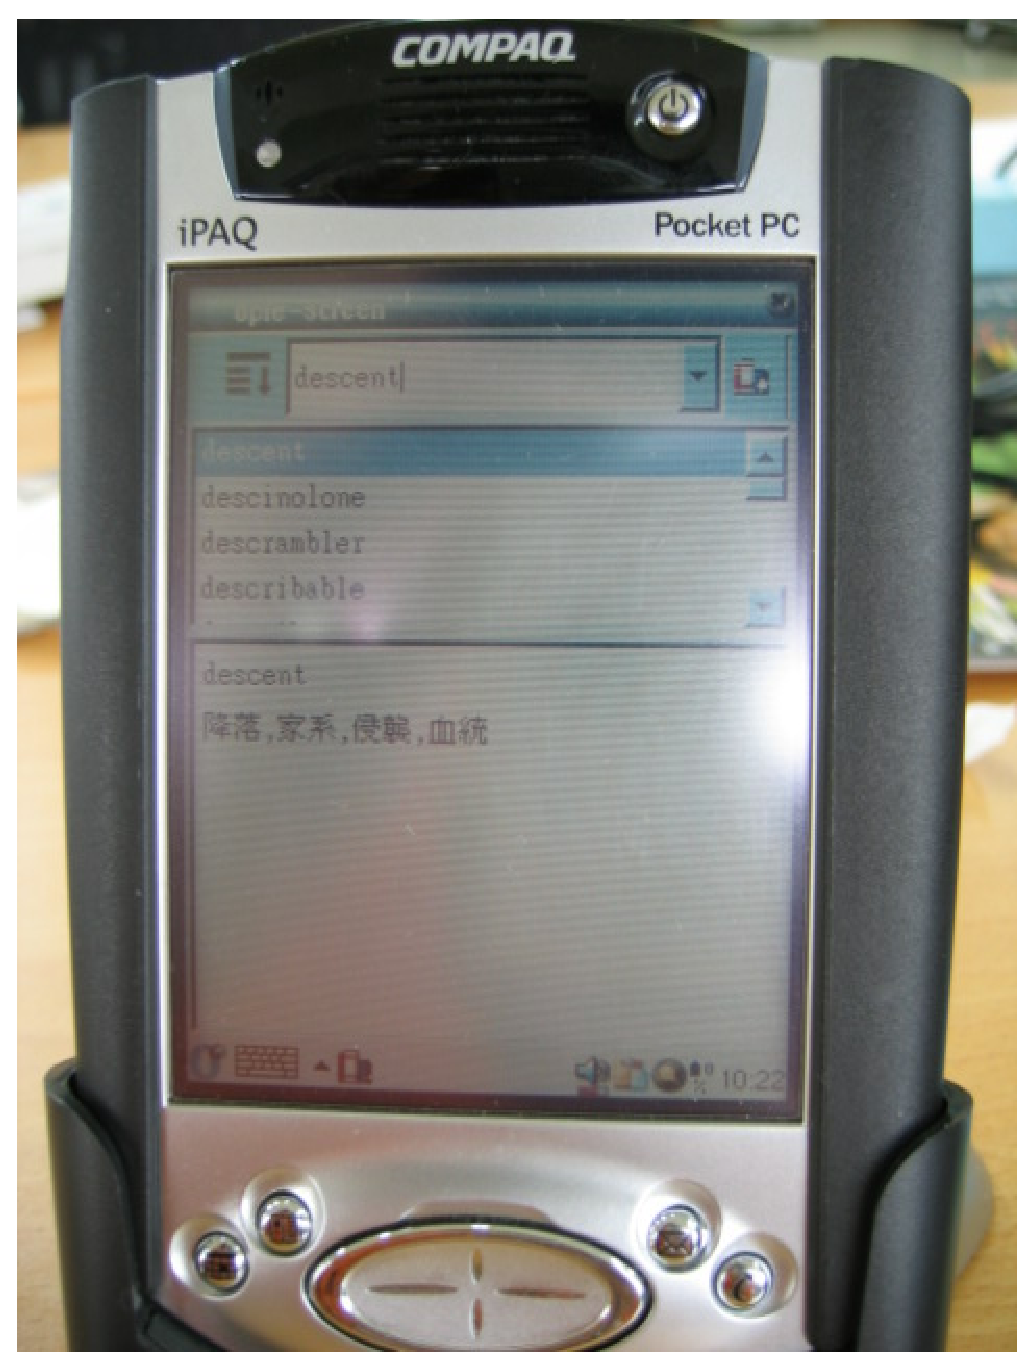
\includegraphics[scale=0.3]{eps/zbedic-0.9.5.eps}
\caption{zbedic-0.9.5}
\end{figure}

\section{讓 IPAQ 透過 usb 上網快速導覽}
usb/serial line 可以同時接上。
我是用 minicom 來做以下的設定,
也可以用 konsole 來做設定。
需要 usbnet 這個 module。

in pc

\begin{verbatim}
/sbin/ifconfig usb0 192.168.129.200 broadcast \
192.168.129.255 netmask 255.255.255.0
echo 1 > /proc/sys/net/ipv4/ip_forward
/sbin/iptables -t nat -A POSTROUTING -o eth0 -s 192.168.129.201 -j MASQUERADE
\end{verbatim}

\noindent
in ipaq:
\begin{verbatim}
ifconfig usbf 192.168.129.201
route add -net default gw 192.168.129.200
\end{verbatim}
在 /etc/resolv.conf 加入 dns
\begin{verbatim}
nameserver 168.95.1.1
\end{verbatim}



我安裝的 familiar 0.7.2 有 sshd 可以用,
當連線設定完成後, 就可以用 ssh 登入了。
擺脫慢慢的 minicom 吧!

以下是我參考的網站資料:
\cite{ethernet_usb}, \cite{ZAURUS}, \cite{usb_driver}


\section{Embedded Konqueror}
需要 
\begin{verbatim}
export KDEDIR=/opt/Qtopia/
\end{verbatim}

\$KDEDIR/shaer 需要有
\begin{verbatim}
apps        config 
\end{verbatim}
這是 embedded konqueror 原始程式提供的。


\begin{figure}[htbp]
\centering
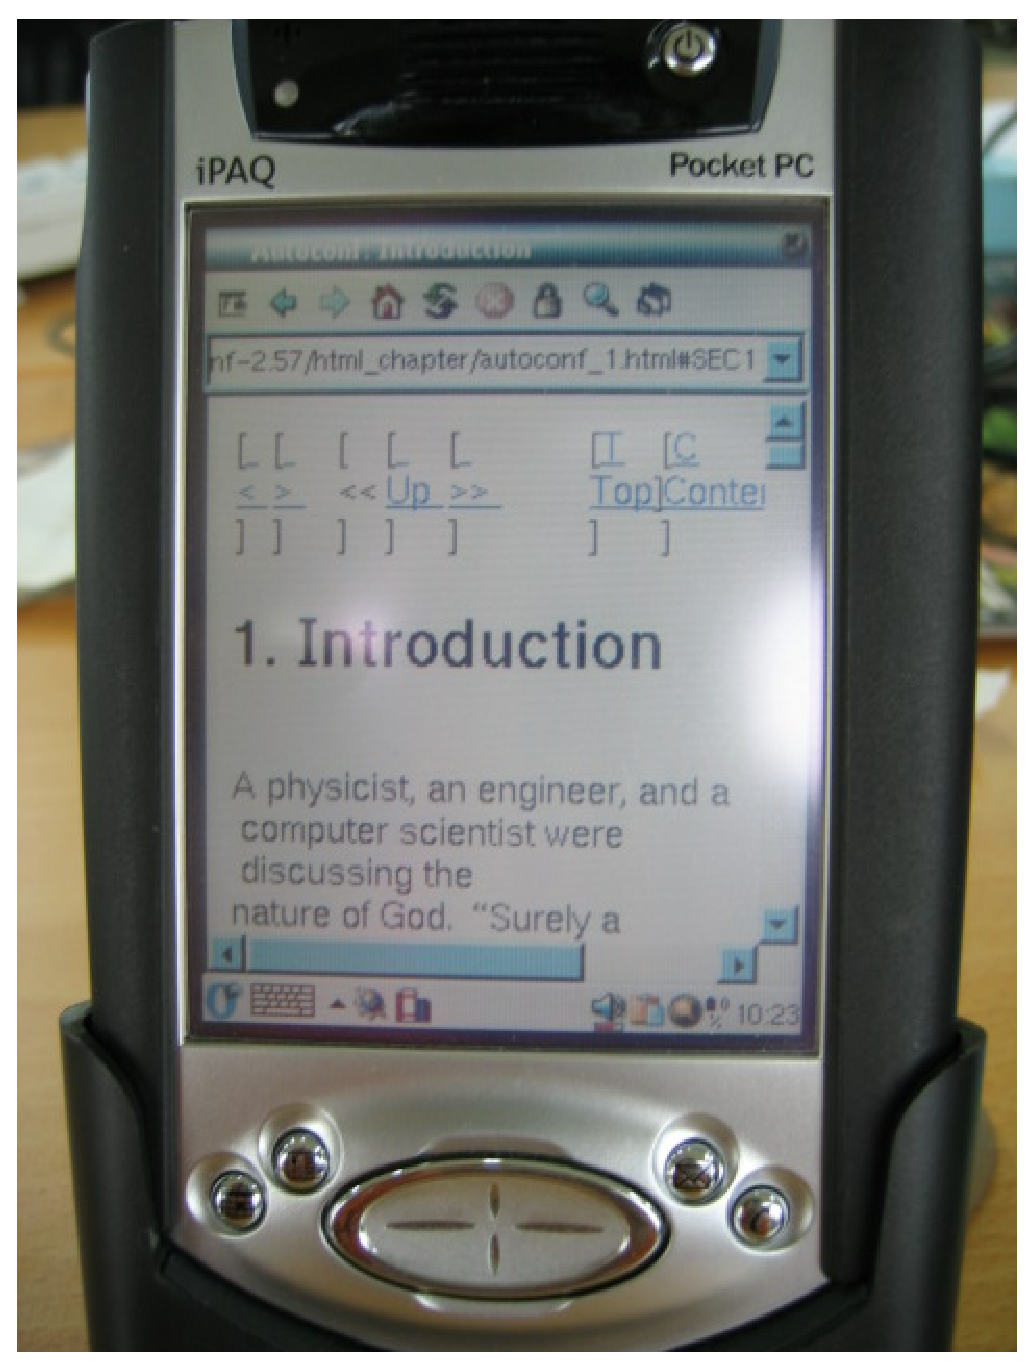
\includegraphics[scale=0.3]{eps/konqueror.eps}
\caption{konqueror-embedded-snapshot-20030705}
\end{figure}

這幾個版本可以編譯成功。
\begin{verbatim}
konqueror-embedded-snapshot-20030705
konqueror-embedded-snapshot_20020127
\end{verbatim}
請參考我網頁中的 cross compile for arm (with mmu) software 連結。

\section{ipkg 常用的 option}
/etc/ipkg.conf
src f http://familiar.handhelds.org/releases/v0.7.2/base/armv4l
src o http://opie.handhelds.org/feed/ipaq/stable/latest/
ipkg command
\begin{verbatim}
-force-reinstall        
-force-overwrite 
-nodeps
-recursive
list // list packages
</pre>
\end{verbatim}

\section{中文輸入法}

\begin{figure}[htbp]
\centering
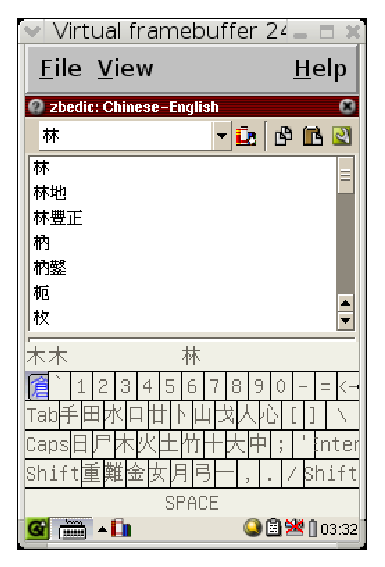
\includegraphics[scale=0.9]{eps/changjei.eps}%
\hspace{1in}%
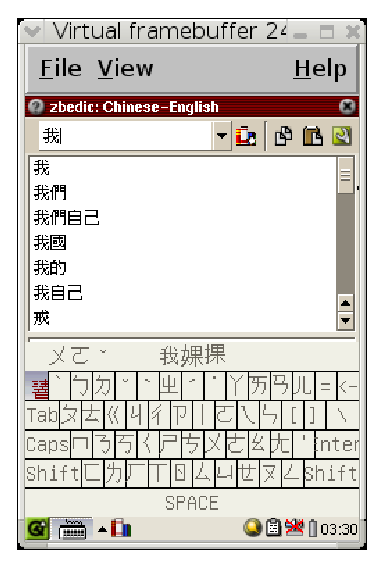
\includegraphics[scale=0.9]{eps/phonetic.eps}
\caption{倉頡, 注音輸入法}
\end{figure}

 目前在 QTOPIA/OPIE 環境我測試的 zbedic/text editor 可以接受此輸入法,
 text editor 要選擇可以秀出中文的字型。
 其餘的程式可能需要修改才能正確輸入中文。
 這是使用倚天的輸入法表格 phonetic.tab, changjei.tab,
 請將這兩個檔案放到 \$QPEDIR/plugins/inputmethods 下,
 否則可能造成 QTOPIA 無法啟動。 	
 由於這兩個檔案是商業軟體所以就要麻煩大家自己去找了,
 在倚天中文這套軟體可以找到。
 編譯方法: 設定好 QTDIR, QPEDIR 環境變數,
 make 即可,
 arm 版本 \verb|make CXX=arm-linux-g++| 即可。
 這個程式寫得很不好, 只是擁有基本功能,
 若看到原始碼覺得好笑的話, 那就笑出來吧!\verb+^_^+
 內傷就不好了。
 若是屬於我可以決定的部份採用 BSD license。

\section{qembed}

這是可以把小圖檔轉成 c code (.h) 的形式插入到程式碼內。

\begin{verbatim}
qembed up.png right.png  left.png > embed_pic.h
\end{verbatim}
會產生一個 \verb+embed_pic.h+ 的檔案。

使用範例:
先 \verb+#include "embed_pic.h"+
然後
\begin{verbatim}
setPixmap(qembed_findData("up"));
QPixmap(qembed_findData("en.png");
\end{verbatim}

可以藉由使用 \verb+qembed_findData()+ function 來產生所指定圖檔的 
QPixmap。這樣就可以不用將圖檔帶著跑了。

\section{建立 jffs2 image}
參考網址: \cite{make_jffs2}

How to create a custom jffs2 image for the iPAQ
Familiar Version: .5, .5.1
\begin{enumerate}
\item Download the latest jffs2 *.tar.gz file for familiar.
\item Update the files you want to change
  (i.e: Update the modules directory with the latest modules)
\item Make sure all files are owned by root Execute \\
\verb+'find ./ -print | xargs chown root.root'+ from the root of your jffs2 image.
\item Obtain mkfs.jffs2 from here.
\item Execute \verb+mkfs.jffs2 -o outfile.jffs2 -d directory -p -e 0x40000+
i.e: \verb+mkfs.jffs2 -o test.jffs2 -d task-bootstrap -p -e 0x40000+
Note: 0x20000 is for mono Ipaqs (31xx's), 0x40000 is for color ipaqs(36xx's, 37xx's, 38xx's).
\end{enumerate}

ex: 
\begin{verbatim}
mkfs.jffs2 -r ipaq-3870 -e 0x40000 -o ipaq-3870.jffs2
\end{verbatim}


\section{安裝 Intimate Linux}\label{intimate}
簡單的說就是把 debian for arm 裝到 IPAQ。
目前 support IPAQ 36XX, 38XX。
是將 linux 裝到 cf, ide 等裝置。
有新舊兩種裝法, 舊的需要 familiar 0.5,
新的方法可以使用 dual boot,
不過我若保存 wince 則不能成功開到 linux,
原因是開機時去系統會去 mount wince flash 但因為並不是 jffs2 所以就 hang 在那裡,
我看到一堆的 jffs2 error message。
所以我把 familiar 0.5 裝回去就可以開到 cf 的 linux。
或是把 \verb+/etc/fstab+
\begin{verbatim}
/dev/mtdblock/1 /       jffs2   defaults 1 1
\end{verbatim}
註解起來即可 dual boot, 正常的進入 Intimate Linux。
因為 wince 不是使用 jffs2, 所以在 mount \verb+/dev/mtdblock/1+
會有問題, 但是若重新開機, wince 資料會消失不見, 包括新裝的軟體。
導致 dual boot 意義不大, 這是 boot loader 的以知 bug。
原因是 wince 有使用 dram 來存某些資料。
若是開到 linux (cf 背夾) 在重新開到 WINCE,
藍芽的使用會有問題。


\begin{figure}[htbp]
\centering
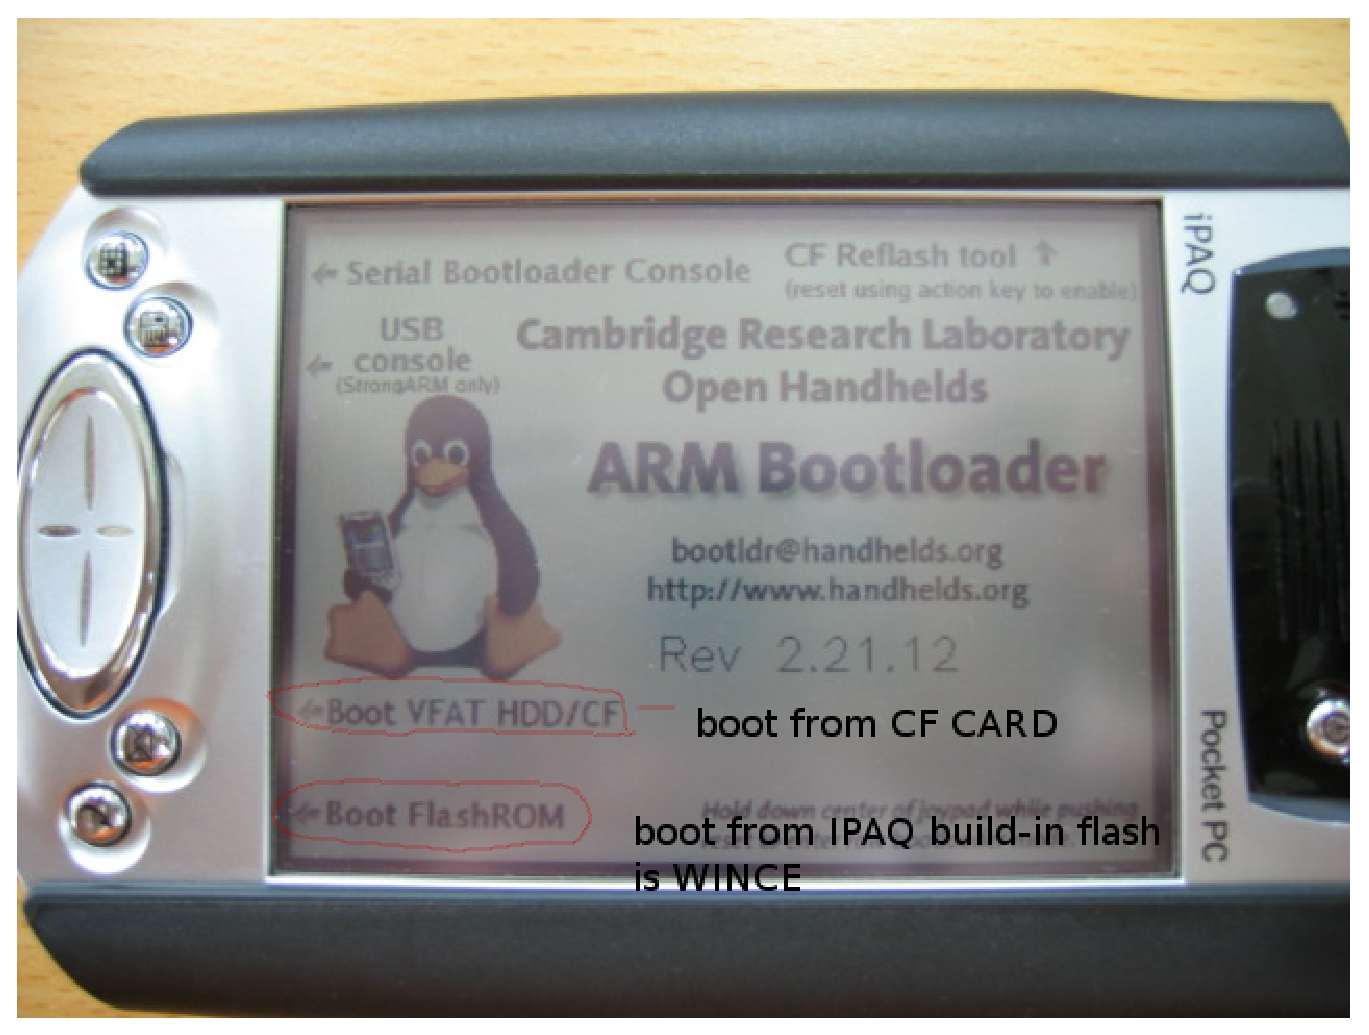
\includegraphics[scale=0.5]{eps/bootloader.eps}
\caption{IPAQ Boot Loader 畫面}
\end{figure}

\begin{figure}[htbp]
\centering
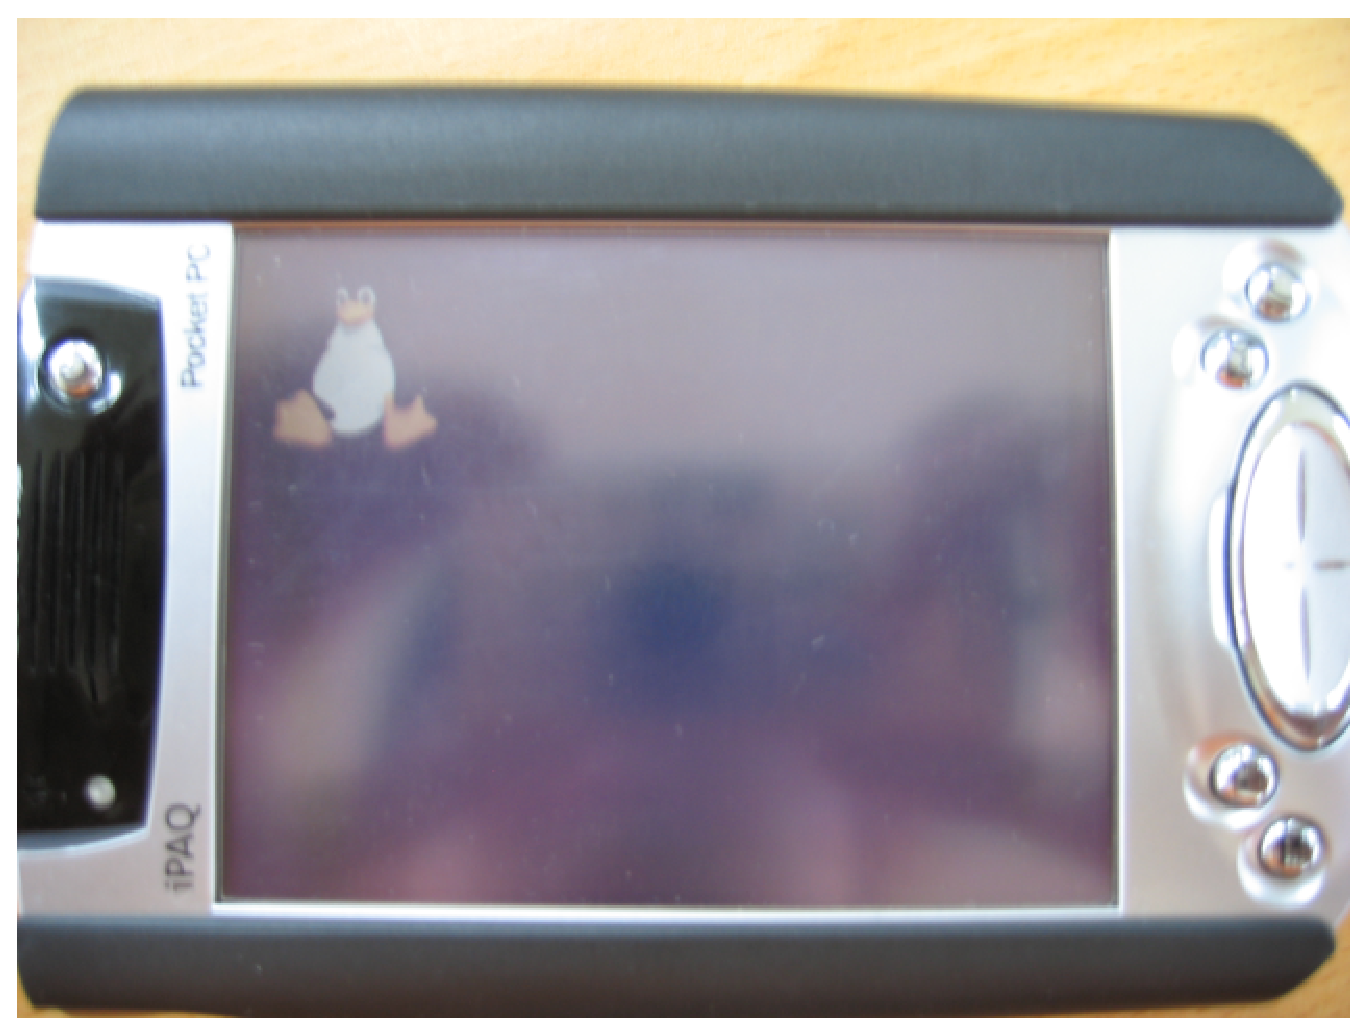
\includegraphics[scale=0.5]{eps/booting_1.eps}
\caption{IPAQ Linux Booting 1}
\end{figure}

\begin{figure}[htbp]
\centering
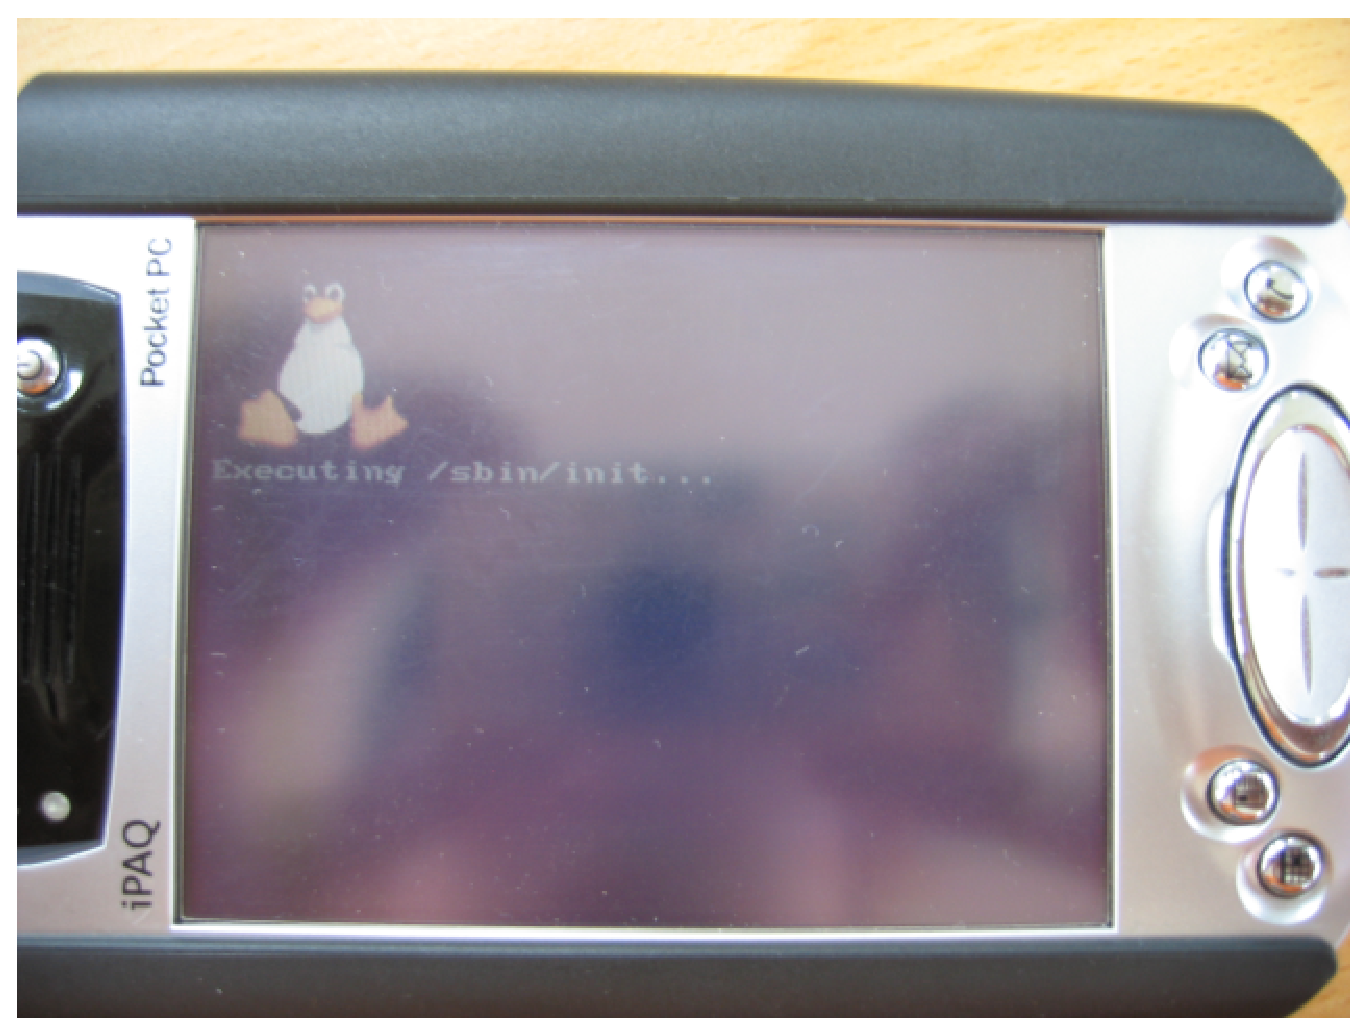
\includegraphics[scale=0.5]{eps/booting_2.eps}
\caption{IPAQ Linux Booting 2}
\end{figure}

參考: \cite{intimate}

\subsection{安裝/編譯 familiar kernel}
因為 intimate 的 kernel 抓不到 mmc/sd card, 有 mmc/sd kernel module,
但是無法 mount sd card (這是因為 Intimate Linux 附的 kernel 不夠新) 。
所以我去下載 familiar 最新的 kernel。

\subsubsection{download familiar kernel}
先到這裡看看有那些 kernel 版本
\verb+http://handhelds.org/cgi-bin/cvsweb.cgi/linux/kernel/+

\begin{verbatim}
export $TAG=K2-4-19-rmk6-pxa1-hh37-4
http://www.handhelds.org/handhelds-faq/development.html
bash$ export CVSROOT=:pserver:anoncvs@cvs.handhelds.org:/cvs
bash$ cvs login
password: anoncvs
cvs checkout -r $TAG linux/kernel
\end{verbatim}
下載指定的 branch 版本。

README.HANDHELDS 必讀, 以獲得如何 comcpile kernel 的方法。

\subsection{ipaq bootloader 的參數檔}
params 紀錄著 ipaq bootloader 的參數,
將 params 裡的內容修改成

\begin{verbatim}
set linuxargs
console=ttySA0
\end{verbatim}

可以在 ipaq 螢幕看見開機訊息。
familiar distribute 也可以找到此檔, 在 \verb+/boot/params+
其內容為:
\begin{verbatim}
set linuxargs "root=/dev/mtdblock1 init=/linuxrc noinitrd console=none"
\end{verbatim}

\subsection{用 apt-get 安裝 opie}
不過經我測試, 這裡附的 qt-embedded library 並不支援 touch pannel,
所以還是自己 compile 一份吧!
\begin{verbatim}
apt-get install op-fb
\end{verbatim}
打完收工。
\begin{verbatim}
/etc/init.d/opie
export QTDIR=/usr/share/qt
\end{verbatim}
設定有錯
\begin{verbatim}
export QTDIR=/usr/share/qte2
\end{verbatim}
才對

\subsection{apm 設定}
可以用用看 apmd, 一樣 apt-get install apm 即可。
需要建立 \verb+/dev/apm_bios+
\verb+mknod /dev/apm_bios c 10 134+
或是作一個 symbolic link
\begin{verbatim}
ln -s /dev/misc/apm_bios /dev/apm_bios
\end{verbatim}

需要 insmod apmd.o kernel module。

這樣才能按電源按鍵進入 suspend mode。

\subsection{getty 重新設定}
\verb+/etc/inittab+
修改成
\begin{verbatim}
T0:23:respawn:/sbin/getty ttySA0 115200 vt100
\end{verbatim}
這樣 run opie, button 才會正常。
否則會跟 console 搶 button。


\section{IPAQ 3870 改裝記}

尋尋覓覓了一年, 終於在 yahoo 拍賣網站以 7500 買了一部 3870,
有 CF 背夾 (未拆封), 車充, 還蠻新的, 
有藍芽功能。
不過 7500 不能算是便宜,

玩了 win ce 幾天後, 開始掙扎要不要換成 familiar (linux os),
心中幾經掙扎, 以戒慎恐懼的心情開始了,
最重要的是 boot load, 嗯! 看看文件, download 檔案,
在看到小企鵝的 boot load 的畫面時, 心中一塊大石頓時放了下來。
要不然我的 IPAQ 3870, 就毀了。 \verb+~^_^~+
好! 開始安裝 dual boot, 把 familiar 裝在 cf,
這樣就可以雙開機了。

很遺憾, 由於看錯文件了, 所以 win ce 被我蓋掉了,
現在只剩下 familiar, win ce 不見了。 我是安裝 opie 的環境,
感覺還不錯。

至於要 dual boot,
可以參考 \ref{intimate}。

由於有備份 win ce bootload, win ce 本身, 所以理論上是可以把
win ce 裝回去的, 只要在 bootloar 提示符號下
\begin{verbatim}
load root
\end{verbatim}
選擇 YMODEM, 載入備份的 wince image file, 即可回復到 
wince 環境。

\begin{verbatim}
load load bootldr
\end{verbatim}
選擇 YMODEM, 載入備份的 wince bootloader (\verb+saved_bootldr.gz+),
即可回復 wince bootloader。

以上命令在我的 iPAQ 3870 可以正常執行。

\section{SD CARD in IPAQ 3879}
為了在 wince 和 linux 共用 SD CARD,
我使用了以下的方法造出檔案系統。
先用讀卡機刪除所有 SD CARD partition,
插入 WINCE 讓 WINCE format。
也就是不建立 sdc1, sdc2 ... 這些 partitions,


在 linux 以下列指令 mount:
\begin{verbatim}
mount -t vfat -o iocharset=cp950 /dev/sdc /mnt/cf
\end{verbatim}

這樣長檔名和中文就沒問題了。

\section{IPAQ 3870 的維修}
我的 iPAQ 3870 在換電池時, 電池排線被我弄壞了, 
由於找不到那裡可以修理, 所以直接送到 HP 維修。

目前已經修理好了, 我在 2005/07/13 送到 HP 維修中心,
2005/07/28 收到, 費用很貴,
加運送費用總共 1575, 才一條電池排線
竟然要這麼貴。

HP 維修中心: 台北市信義路 5 段 106 號 B1

        維修電話: 02-87228000
                  0800010055

        我忘了個別的功能,
        有關維修的問題都可以打。

希望大家好好愛惜自己的 PDA, 維修好貴阿。

對了, 基本運送費用 300 是一定要付的。

\section{我 IPAQ 3870 的保護殼}
2005/06/23 拿到在 Yahoo 拍賣買的 IPAQ 3870 保護殼,
花了我 1150, 據說可以防震防水。除了厚重點外,
看起來蠻討喜的。

\begin{figure}[htbp]
\centering
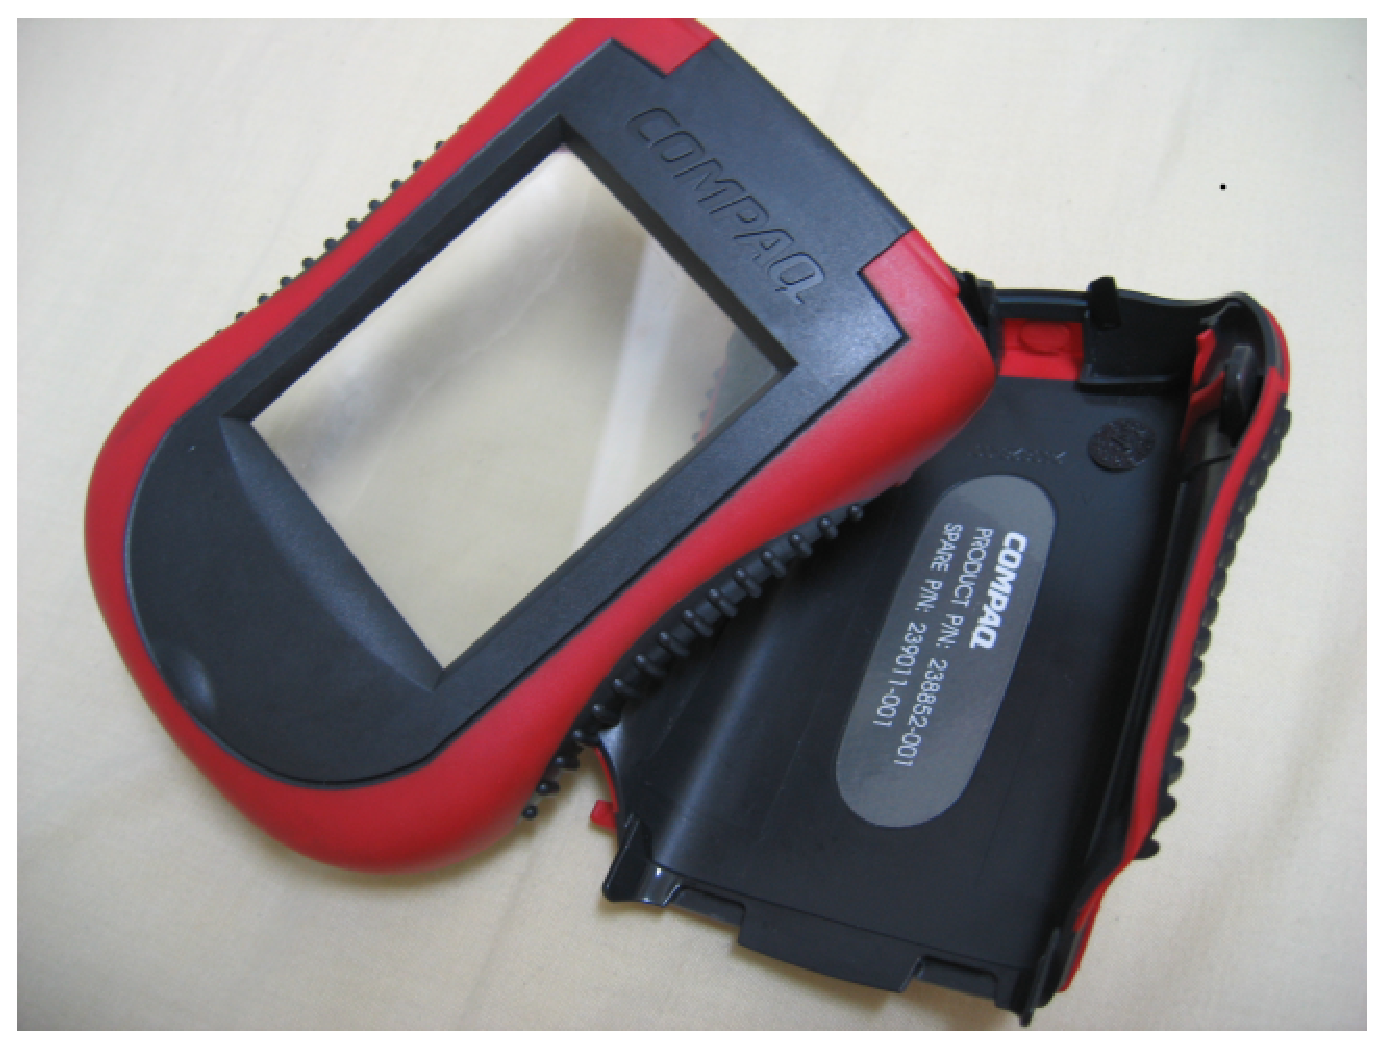
\includegraphics[scale=0.4]{eps/shell_1.eps}
\caption{保護殼 1}
\end{figure}

\begin{figure}[htbp]
\centering
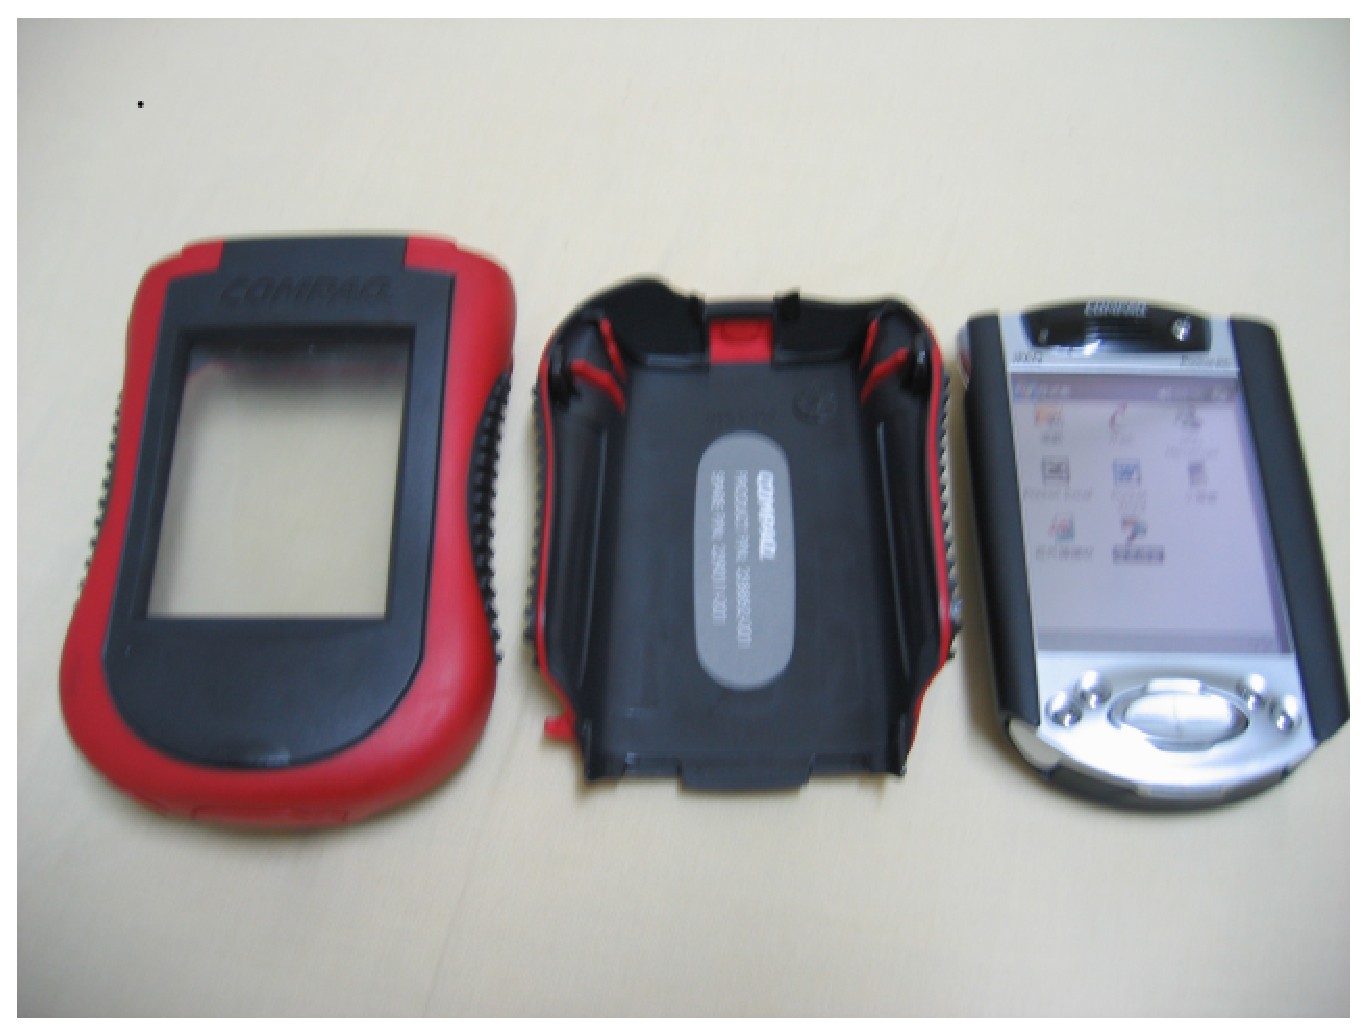
\includegraphics[scale=0.4]{eps/shell_2.eps}
\caption{保護殼 2}
\end{figure}

\begin{figure}[htbp]
\centering
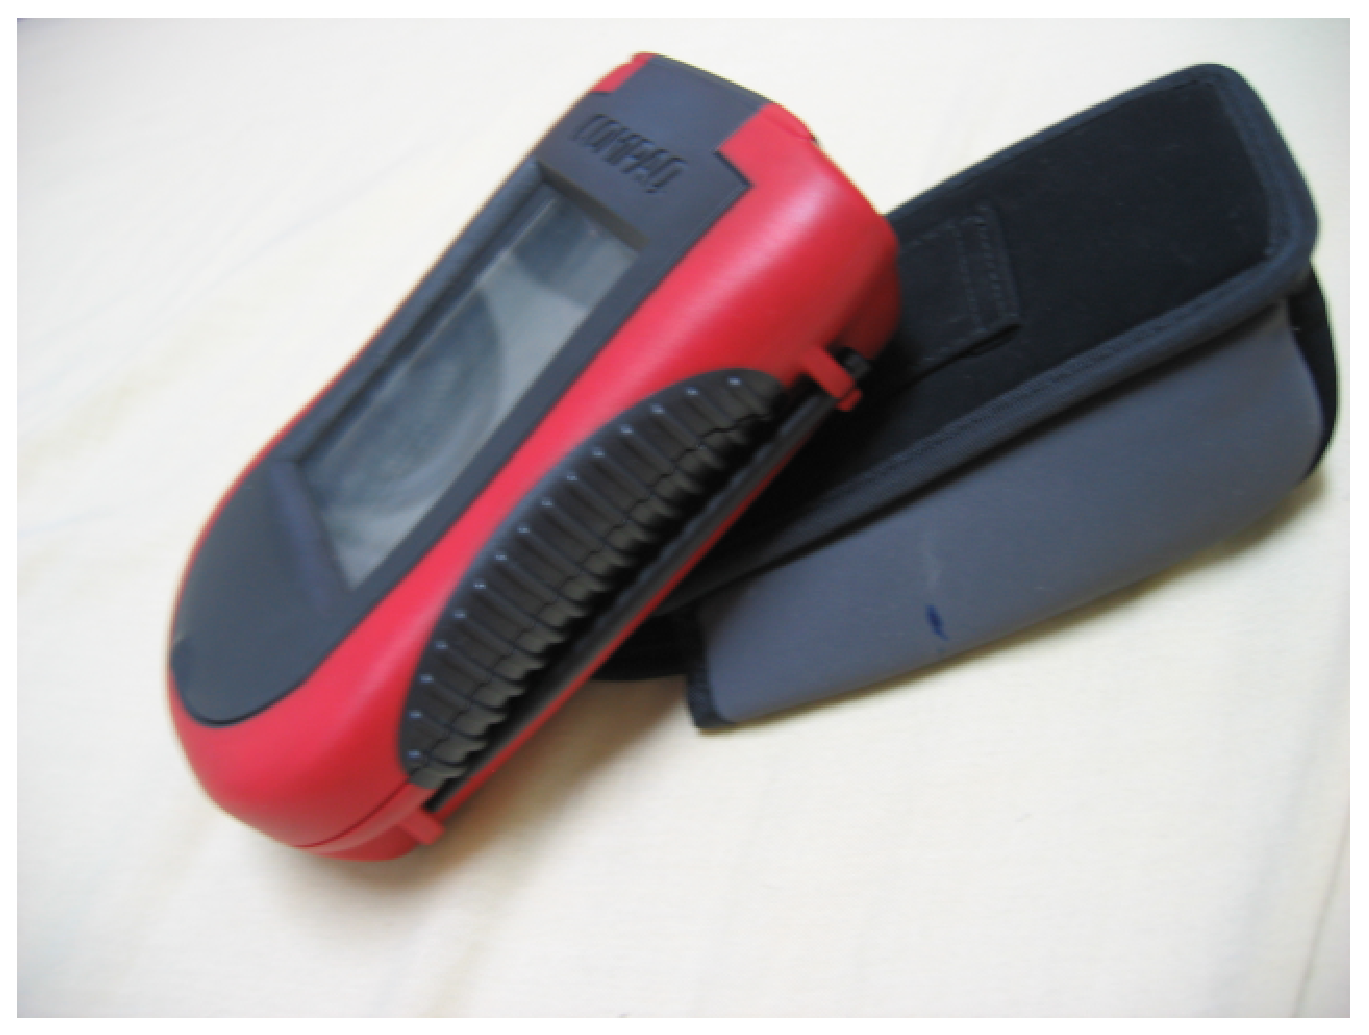
\includegraphics[scale=0.3]{eps/shell_5.eps}
\caption{保護殼 3}
\end{figure}

\begin{figure}[htbp]
\centering
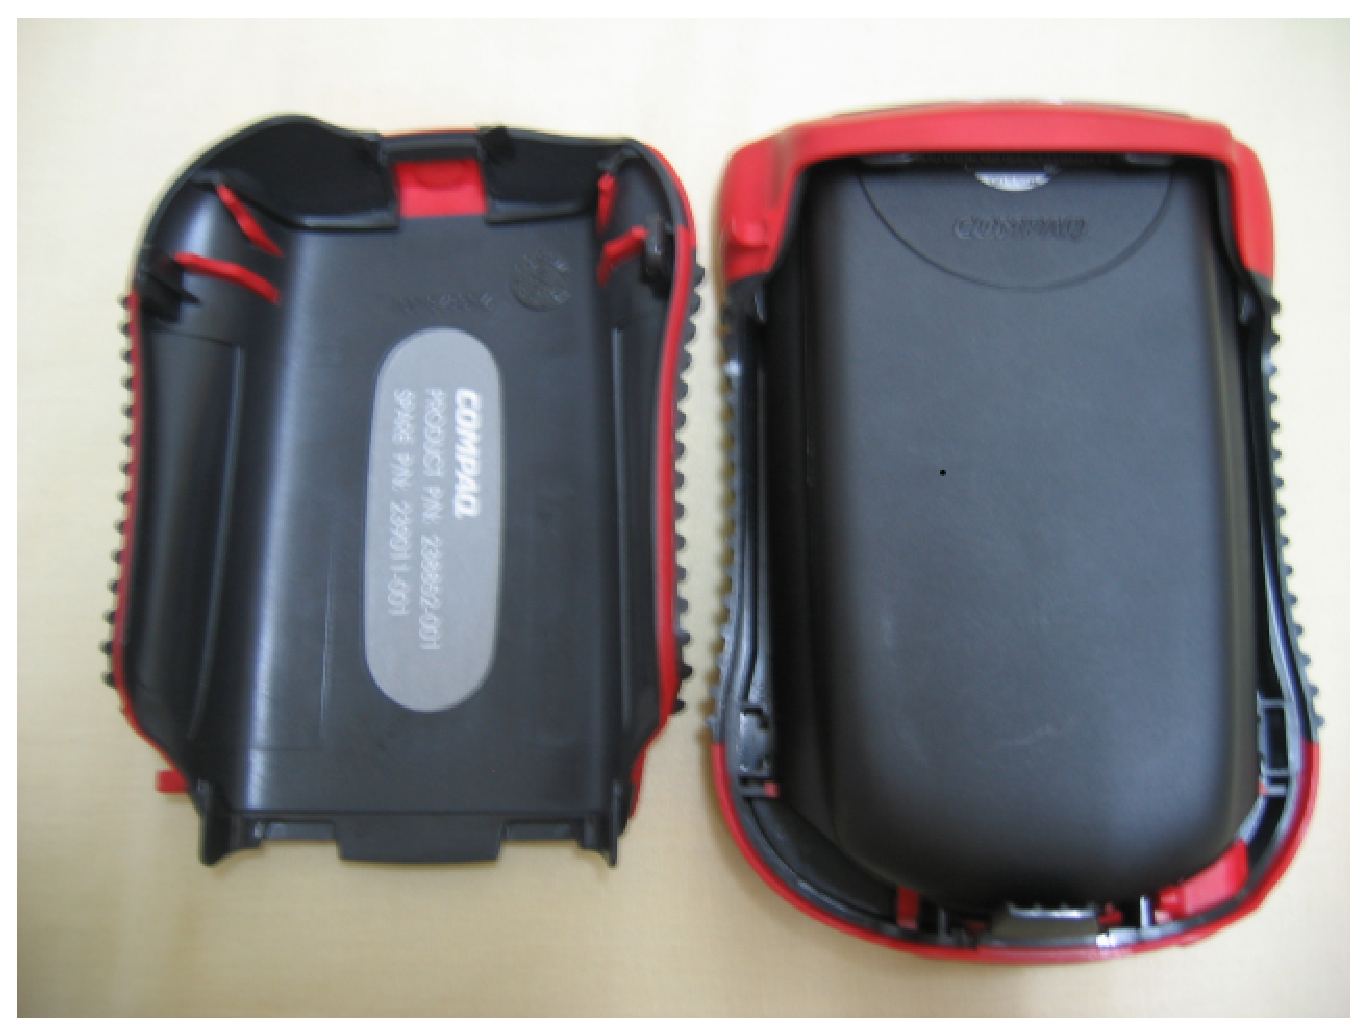
\includegraphics[scale=0.3]{eps/shell_3.eps}%
\hspace{0.5cm}%
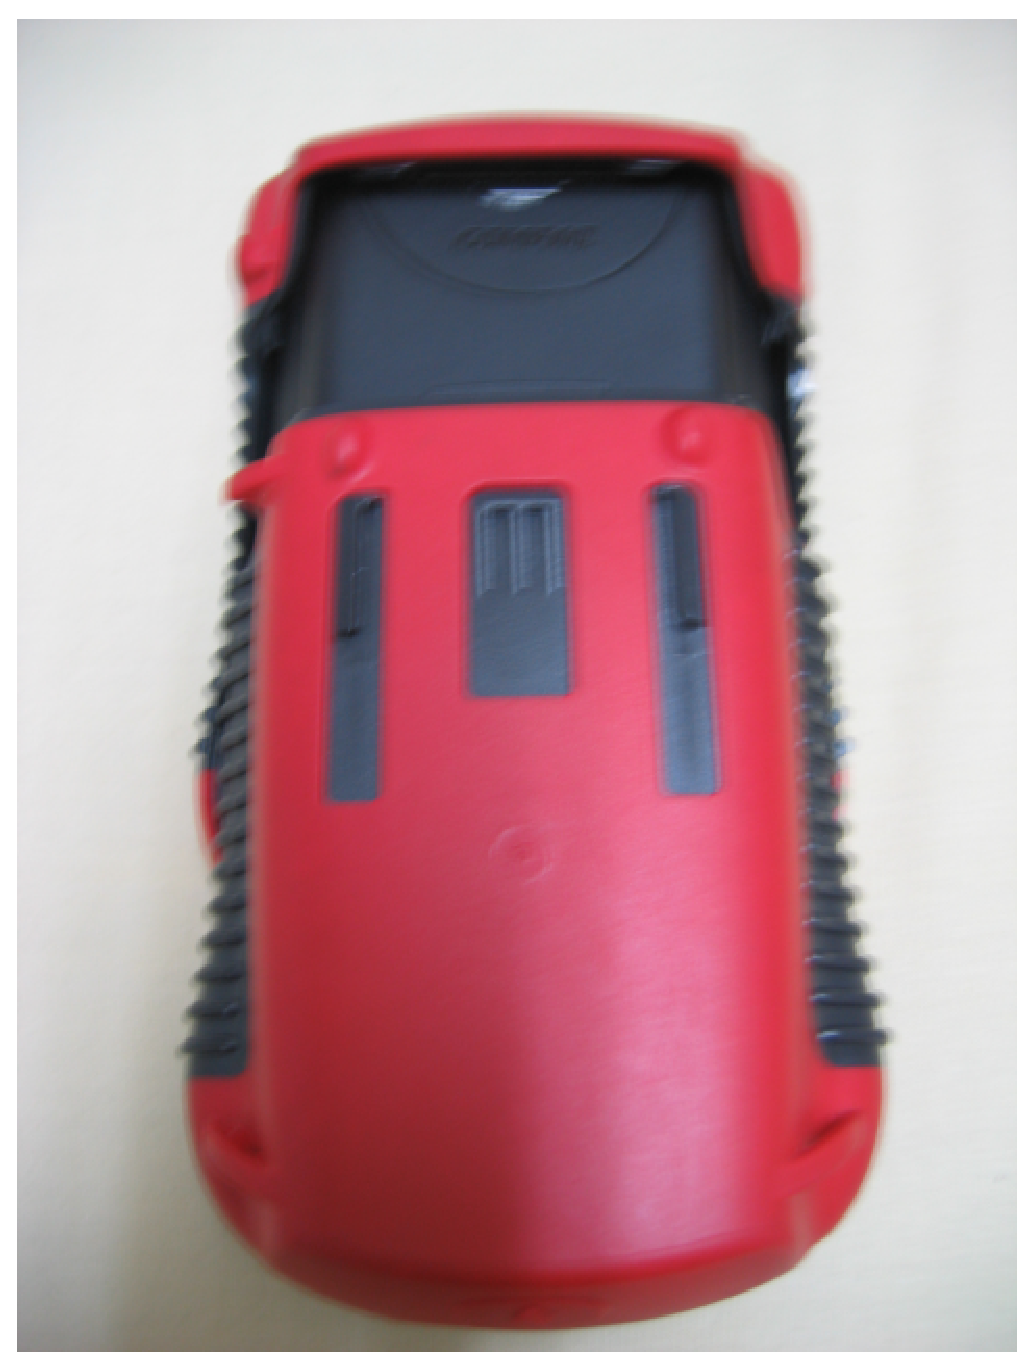
\includegraphics[scale=0.3]{eps/shell_4.eps}
\caption{將 IPAQ 裝入保護殼 1}
\end{figure}


\begin{figure}[htbp]
\centering
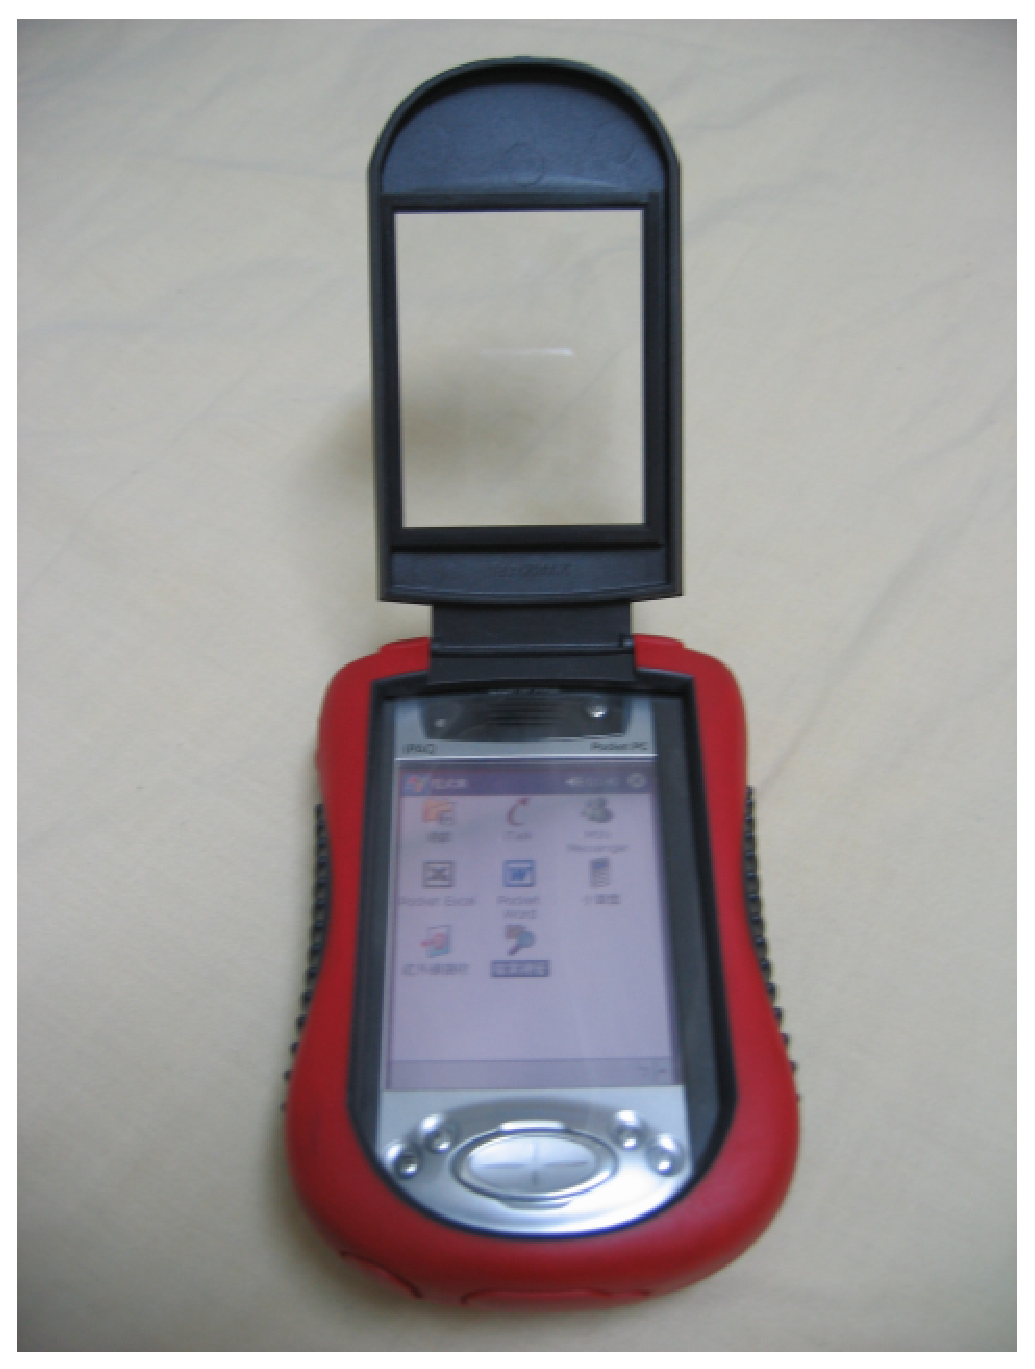
\includegraphics[scale=0.35]{eps/shell_6.eps}%
\hspace{0.5cm}%
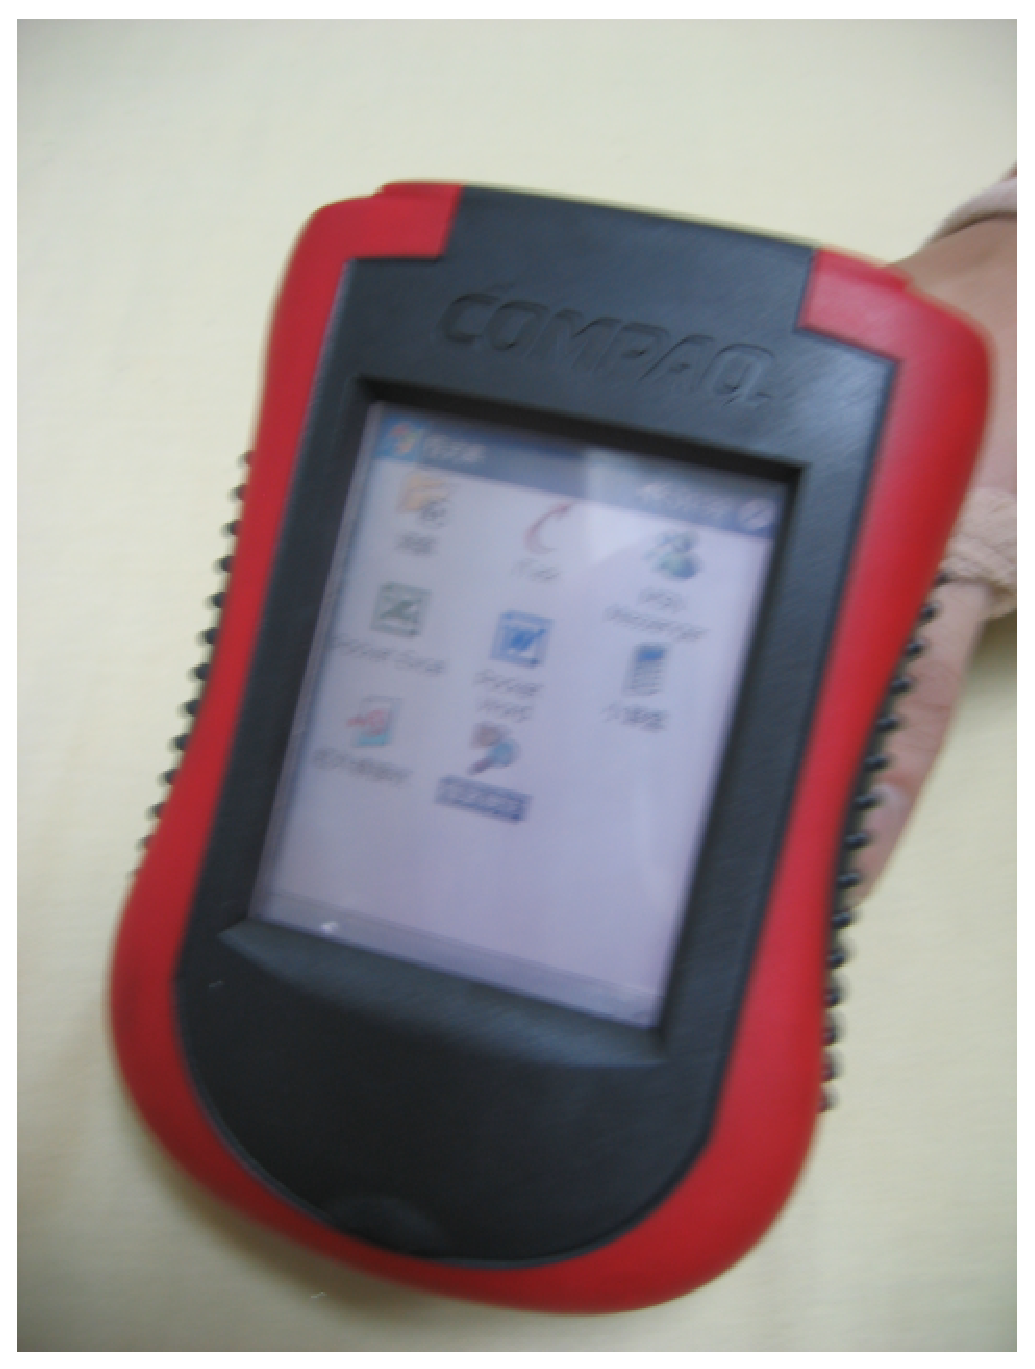
\includegraphics[scale=0.35]{eps/shell_7.eps}
\caption{將 IPAQ 裝入保護殼 2}
\end{figure}

由於實在是很厚, 覺得像是 IPAQ 3870 的棺材。

\section{opie Dependencies}
\begin{verbatim}
opie-1.1.9
Have Libetpan >= 0.33pre
Have libpcap>=0.7.2
Have sqlite>=3.0.7
Have libxine>=1.0rc6
Have libipkg>=0.99.120
Have libsdl12andsdlimage
Have libsword>=1.5.0
Have bluezlibrary
Have freetype2
\end{verbatim}


\begin{verbatim}
$OPIEDIR/opie-1.2.0/libopie2/opiecore/device
\end{verbatim}
有一些和 device 有關的程式碼,

\begin{verbatim}
ODevice::inst ( )-> setDisplayStatus ( false );
\end{verbatim}

可以關掉背光。

opieplayer2 需要把 lo 網路裝置設起來,
要不然 run 不起來。

\begin{verbatim}
用 opie-1.2.0 patch qt-2.3.10

patching file src/iconview/qiconview.cpp
patching file src/iconview/qiconview.h
patching file src/kernel/qgfxraster_qws.cpp
patching file src/kernel/qwindowsystem_qws.cpp
patching file src/kernel/qwsdecoration_qws.h
patching file src/tools/qcstring.h
patching file src/tools/qstring.cpp
patching file src/widgets/qcommonstyle.cpp
patching file src/widgets/qlistview.cpp
patching file src/widgets/qtoolbutton.cpp
patching file src/widgets/qtabbar.cpp
\end{verbatim}


\begin{verbatim}
make apidox
\end{verbatim}

\parindent=0cm
\parskip=20pt

可以產生 opie document。
\end{CJK}{UTF8}


\begin{thebibliography}{99}
\bibitem{ethernet_usb} http://www.ruault.com/Zaurus/ethernet-over-usb-howto.html
\bibitem{ZAURUS} http://paar.kh.edu.tw/MT-blog/C700/archives/000026.html
\bibitem{usb_driver} http://www.linux-usb.org/usbnet/
%\bibitem{makeqpf} http://www.zauruszone.farplanet.net/wiki/index.php?TTF%20To%20QPF%20HOWTO
\bibitem{make_jffs2} \verb+http://internet2.motlabs.com/ipaq/howto/custom_jffs2_ipaq.htm+
\bibitem{intimate} \verb+http://intimate.handhelds.org/news.html+
\end{thebibliography}
  
\end{document}
